\documentclass[a4j,titlepage]{jsarticle}

\usepackage[dvipdfmx]{graphicx,xcolor}
\usepackage[top=20truemm,left=25truemm,right=25truemm]{geometry}
\usepackage{amsmath}
\usepackage{here}
\usepackage{comment}
\usepackage{url}
\usepackage{plistings}
\usepackage{tikz}
\usepackage[framemethod=tikz]{mdframed}

\renewcommand{\lstlistingname}{リスト}

\newcommand{\chuo}[1]{\multicolumn{1}{|c|}{#1}}
\newcommand{\inpt}[1]{\underline{#1}\,\setlength{\fboxsep}{1pt}\fbox{\small ↓}}
\newcommand{\bvec}[1]{\mbox{\boldmath $#1$}}

\lstdefinestyle{C}{
  language=C,
  basicstyle=\small\ttfamily,
  keywordstyle=\color[HTML]{0000E0},
  stringstyle=\color[HTML]{A31515},
  commentstyle=\upshape\color[HTML]{008000},
  frame=trbl,
  framesep=5pt,
  columns=[l]{fullflexible},
  numbers=left,
  xleftmargin=3zw,
  lineskip=-0.2ex,
  breaklines=true,
  showstringspaces=false,
  tabsize=4,
  keepspaces=true
}

\lstdefinestyle{make}{
  language=,
  basicstyle=\small\ttfamily,
  keywordstyle=\color[HTML]{0000E0},
  stringstyle=\color[HTML]{A31515},
  commentstyle=\upshape\color[HTML]{008000},
  frame=trbl,
  framesep=5pt,
  columns=[l]{fullflexible},
  numbers=left,
  xleftmargin=3zw,
  lineskip=-0.2ex,
  breaklines=true,
  showstringspaces=false,
  tabsize=4,
  keepspaces=true
}

\lstdefinestyle{text}{
  language=,
  basicstyle=\ttfamily,
  frame=trbl,
  framesep=5pt,
  columns=[l]{fullflexible},
  xleftmargin=3zw,
  lineskip=-0.2ex,
  showstringspaces=false,
  tabsize=4,
  keepspaces=true
}

\mdfsetup{
  skipabove=5pt,
  innertopmargin=10pt,
  innerbottommargin=10pt,
  roundcorner=10pt,
  font=\ttfamily
}


\begin{document}


\begin{titlepage}
  \title{\huge{工学実験実習V} \\ \LARGE{---MPI---}}
	\author{学籍番号:16426 \\ 5年 電子情報工学科 24番 \\ 福澤 大地}
	\date{提出日 : 2020年10月19日}
  \maketitle
\end{titlepage}


\section{目的}
MPI (Message Passing Interface)を用いて、複数のCPU間で通信を行いながら、
並列計算を行うプログラムを作成する。
その上で、並列計算を行うと通常に比べどれほどの高速化を図れるか、
並列計算に適したアルゴリズムとはどのようなものなのかなどを検証する。


\section{実験環境}
プログラムの開発、実行を行った環境を表\ref{tb:kan}に示す。
表\ref{tb:kan}と同様の環境のコンピュータ44台が同一ネットワーク内に接続されており、
公開鍵認証方式でこれらのコンピュータとSSH通信を行える環境で実験を行った。

\begin{table}[H]
  \centering
  \caption{実験環境}
  \label{tb:kan}

  \begin{tabular}{|l|l|}
    \hline
    CPU & Intel Core i5-6600 @ 3.3GHz \\ \hline
    メモリ & 8GB \\ \hline
    OS & Ubuntu 14.04 LTS \\ \hline
    システム & 64bit \\ \hline
    コンパイラ & GCC 4.8.4 \\ \hline
    MPIライブラリ & Open MPI 1.10.2 \\ \hline
  \end{tabular}
\end{table}


\section{MPIとOpen MPIについて}
MPIとは、並列計算を行うために標準化された規格である。
これを用いることにより、1個のCPUで行っていた計算を複数のCPUで分散して行えるようになる。

Open MPI \cite{bib:1} は、MPIに準拠したライブラリの1つであり、Unix上で利用できる。
MPIのライブラリは他にもMPICH \cite{bib:2} などがあるが、本実験ではOpen MPIを使用する。


\section{実行方法}
プログラムのコンパルには\texttt{mpicc}コマンド、実行には\texttt{mpirun}コマンドを使用する。
\texttt{mpicc}コマンドは\texttt{gcc}コマンドと同様の使い方ができ、
\texttt{-Wall}オプションなどを利用することもできる。
\texttt{mpirun}コマンドは、\texttt{-machinefile}オプションで使用するコンピュータの名前とCPUの数が記述されたファイル名を、
\texttt{-np}オプションで使用するCPUの数を指定することで、コンパイルしたファイルを実行することができる。

例えば、``com001'' $\sim$ ``com004''という名前のコンピュータのCPUを1つずつ使用する場合は、
次のように記述されたテキストファイルを適当なファイル名で保存する。
ここでは、ホームディレクトリに``mymachines''というファイル名で保存することとする。

\begin{lstlisting}[style=text]
com001 cpu=1
com002 cpu=1
com003 cpu=1
com004 cpu=1
\end{lstlisting}

そして、``program.c''というファイル名のプログラムをコンパイルし、
先ほど指定した$4$個のCPU実行する場合には次のようなコマンドを入力する。

\begin{lstlisting}[style=text]
$ mpicc program.c
$ mpirun -machinefile ~/mymachines -np 4 ./a.out
\end{lstlisting}

なお、今回の環境では次のようにエイリアスを設定することにより、\texttt{-machinefile}オプションを省略し実行できるようにしてある。

\begin{lstlisting}[style=text]
alias mpirun='mpirun -machinefile ~/mymachines'
\end{lstlisting}


\section{MPIのプログラム}
MPIを用いてプログラムを作成する際は、通常のプログラムとは違い、
今実行しているCPUの数はいくつなのか、自分はどのCPUなのかなどの情報を取得する必要がある。
そのため、MPIのプログラムではリスト\ref{lst:mpi}のように、
前処理を行うプログラムを記述する必要がある。
なお、プログラムの終了時には、必ず\texttt{MPI\_Finalize}関数を呼び出さなければならない。

\lstinputlisting[style=C,caption=MPIのプログラム,label=lst:mpi]{./MPI/test.c}

リスト\ref{lst:mpi}のプログラムを4個のCPUで実行した結果を、リスト\ref{lst:mpikekka}に示す。
リスト\ref{lst:mpikekka}を見ると、\texttt{nsize}に実行しているCPUの数、\texttt{myrank}に自身の番号、\texttt{my\_name}に自身のコンピュータ名が入っていることが分かる。
実行結果が\texttt{myrank}の順番で表示されていないのは、プログラムが各CPU上で同時に実行されているためである。

\lstinputlisting[style=text,caption=MPIのプログラムの実行結果,label=lst:mpikekka]{./MPI/result/test.txt}


\section{課題1}
\subsection{課題内容}
コマンドライン引数から数値$X$を受け取り、$1 \sim X$までの和を$N$台のCPUで求めるプログラムを作成する。
$X$と$N$は任意の自然数とする。

\subsection{プログラムリスト}
課題1のプログラムを、リスト\ref{lst:kadai1}に示す。

\lstinputlisting[style=C,caption=課題1のプログラム,label=lst:kadai1]{./MPI/kadai01.c}

\subsection{プログラムの説明}
\subsubsection{入力値チェック}
$26 \sim 47$行目では、与えられた引数が正しいものであるのかチェックを行っている。

本プログラムでは計算をlong long int型で行っている。
long long int型は64ビットであるため、表せる値の最大値は、$2^{63} - 1$である。
最終的な計算結果がこの範囲に収まっている必要があるので、
入力として許容できる最大値を$n$とすると、式(\ref{eq:range})のようにして求められる。

\begin{align}
  \begin{aligned}
    \sum^{n}_{k = 1} k &= 2^{63} - 1 \\
    \frac{1}{2} n (n + 1) &= 2^{63} - 1 \\
    \frac{1}{2} n^2 + \frac{1}{2} n - 2^{63} + 1 &= 0 \\
    n &\simeq \pm 4.3 \times 10^9
    \label{eq:range}
  \end{aligned}
\end{align}

式(\ref{eq:range})より、$n$が$4 \times 10^9$以内であれば確実にオーバーフローが起こることはないため、
これより大きい値が入力された際はエラーとしてプログラムを終了している。
また、コマンドライン引数が与えられていなかった場合や、
入力された値が0以下であった場合も同様にエラーとしてプログラムを終了している。

\subsubsection{演算}
演算は$51 \sim 53$行目で行っており、\texttt{myrank}$+1$から始め、\texttt{nsize}間隔で数字を足している。
例えば、4個のCPUで実行した場合には、各CPUが担当する数字は次のようになる。
このようにすることで、各CPUで担当する数字の個数と合計のばらつきを少なくしている。

\begin{description}
  \item[CPU 0] 1, 5, 9,  13, 17, $\dots$
  \item[CPU 1] 2, 6, 10, 14, 18, $\dots$
  \item[CPU 2] 3, 7, 11, 15, 19, $\dots$
  \item[CPU 3] 4, 8, 12, 16, 20, $\dots$
\end{description}

\subsubsection{集計}
各CPUで行った計算結果の集計は、55行目の\texttt{MPI\_Reduce}関数で行っている。
このような記述を行うことで、全てのCPUの\texttt{sum}の合計を、
\texttt{ans}に代入することができる。

第4パラメータには演算の種類を指定することができ、56行目の\texttt{MPI\_MAX}では最大値、
57行目の\texttt{MPI\_MIN}では最小値を取得することができる。

\subsubsection{処理時間の計測}
MPIには、過去のある地点からの経過時間を取得する\texttt{MPI\_Wtime}関数が用意されている。
この関数を処理の開始時と終了時に呼び出し、その差分を取ることで、
処理に掛かった時間を計測することができる。
本プログラムでは、49行目で開始時間、59行目で終了時間を取得し、65行目でその差分を表示している。

\subsection{実行結果}
\subsubsection{$1 \sim 54321$の和}
引数に54321を入力し、4個のCPUで実行した場合の結果をリスト\ref{lst:kadai1-1}に、
8個のCPUで実行した場合の結果をリスト\ref{lst:kadai1-1.5}に示す。

\lstinputlisting[style=text,caption=引数に54321を入力した場合の実行結果,label=lst:kadai1-1]{./MPI/result/kadai01-1.txt}

\lstinputlisting[style=text,caption=8個のCPUで実行した場合の実行結果,label=lst:kadai1-1.5]{./MPI/result/kadai01-1.5.txt}

\subsubsection{入力値チェック}
引数を与えなかった場合の結果をリスト\ref{lst:nohiki}, 0以下の数を入力した場合の結果をリスト\ref{lst:underzero}, 
$4 \times 10^9$を上回る数を入力した場合の結果をリスト\ref{lst:toobig}に示す。

\lstinputlisting[style=text,caption=引数を与えなかった場合の実行結果,label=lst:nohiki]{./MPI/result/kadai01-3.txt}

\lstinputlisting[style=text,caption=0以下の数を入力した場合の実行結果,label=lst:underzero]{./MPI/result/kadai01-4.txt}

\lstinputlisting[style=text,caption=最大値以上の数を入力した場合の実行結果,label=lst:toobig]{./MPI/result/kadai01-5.txt}

\subsection{考察}
$1 \sim 54321$の和は$\sum^{54321}_{k = 1} k = 1475412681$である。
これはリスト\ref{lst:kadai1-1}の計算結果と一致するため、正しく計算が行われている。
また、各CPUでの計算結果の最大値と最小値を見比べると、大きな差は見受けられない。
よって、狙い通りCPUによる合計値のばらつきを少なくすることができた。

リスト\ref{lst:kadai1-1.5}を見ると、4個のCPUで実行したリスト\ref{lst:kadai1-1}に比べ、
処理時間が約半分になっている。
このことから、正常に並列計算が行えていると言える。

さらに、リスト\ref{lst:nohiki}--\ref{lst:toobig}を見ると、不正なコマンドライン引数に対して適切なエラーメッセージが表示されている。
よって、正しく入力値のチェックが行えていることが分かる。


\section{課題2}
\subsection{課題内容}
課題1で作成したプログラムを用いて、並列計算の効果を測定する。
CPUの数$N$を変えながら処理時間を測定し、その結果をグラフにして考察する。

\subsection{実行結果}
引数に$4 \times 10^9$を与えた場合について、CPUの数$N$を$1 \sim 30$個に増やしながら処理時間を測定した。
全てのCPUが作業が行われていない状態で測定を行い、それぞれ10回の平均値を取った。

それぞれのCPUの個数についての処理時間についてまとめたものを表\ref{tb:kadai2}に、グラフにプロットしたものを図\ref{fig:kadai2}に示す。

\begin{table}[htbp]
  \centering
  \caption{CPUの個数と処理時間}
  \label{tb:kadai2}

  \begin{tabular}{|r|r|r|}
    \hline
    \chuo{CPU数 [個]} & \chuo{処理時間 [ms]} & \chuo{CPU1個の処理時間に対する短縮率} \\ \hline \hline
     1 & 7663 &  1.00 \\ \hline
     2 & 3842 &  1.99 \\ \hline
     3 & 2572 &  2.98 \\ \hline
     4 & 1929 &  3.97 \\ \hline
     5 & 1544 &  4.96 \\ \hline
     6 & 1289 &  5.94 \\ \hline
     7 & 1113 &  6.89 \\ \hline
     8 &  971 &  7.89 \\ \hline
     9 &  862 &  8.89 \\ \hline
    10 &  780 &  9.83 \\ \hline
    11 &  711 & 10.78 \\ \hline
    12 &  652 & 11.76 \\ \hline
    13 &  613 & 12.49 \\ \hline
    14 &  576 & 13.29 \\ \hline
    15 &  536 & 14.29 \\ \hline
    16 &  492 & 15.58 \\ \hline
    17 &  466 & 16.46 \\ \hline
    18 &  440 & 17.42 \\ \hline
    19 &  415 & 18.48 \\ \hline
    20 &  397 & 19.29 \\ \hline
    21 &  391 & 19.61 \\ \hline
    22 &  370 & 20.71 \\ \hline
    23 &  346 & 22.17 \\ \hline
    24 &  328 & 23.36 \\ \hline
    25 &  319 & 24.05 \\ \hline
    26 &  309 & 24.83 \\ \hline
    27 &  300 & 25.51 \\ \hline
    28 &  296 & 25.91 \\ \hline
    29 &  282 & 27.19 \\ \hline
    30 &  266 & 28.77 \\ \hline
  \end{tabular}
\end{table}

\begin{figure}[H]
  \centering
  \includegraphics[width=12cm]{./MPI/kadai02-result/kadai02.png}
  \caption{CPUの個数と処理時間の関係}
  \label{fig:kadai2}
\end{figure}

\subsection{考察}
図\ref{fig:kadai2}を見ると、反比例のグラフとなっている。
また、表\ref{tb:kadai2}のCPU1個の処理時間に対する短縮率より、おおよそCPUの数の分だけ処理時間の短縮がされていることが分かる。
このことから、課題1のような、ほとんど通信を行わない単純な並列計算を行うと、投入したCPUの数の分だけ効率化が行えると言える。


\section{課題3}
\subsection{課題内容}
$N$個のCPUでモンテカルロシミュレーションを並列処理するプログラムを作成する。
乱数の種はCPUごとに異なるようにする。

\subsection{プログラムリスト}
課題3のプログラムを、リスト\ref{lst:kadai3}に示す。

\lstinputlisting[style=C,caption=課題3のプログラム,label=lst:kadai3]{./MPI/kadai03.c}

\subsection{プログラムの説明}
\subsubsection{入力値チェック}
$30 \sim 55$行目では、与えられた引数が正しいものであるのかチェックを行っている。

本プログラムでは、円を分割したものを各CPUで分担してシミュレーションを行うため、
各CPUでプロットする点は等しい必要がある。
そこで、コマンドライン引数から受け取った値がCPUの個数の倍数でない場合は、エラーとしてプログラムを終了している。
また、コマンドライン引数が与えられていなかった場合や、
入力された値が0以下であった場合も同様にエラーとしてプログラムを終了している。

\subsubsection{シード値の決定}
ランダムな点をプロットするために、各CPUでシード値を決定する必要がある。
通常のプログラムであれば、現在時刻をシード値とするのが一般的であるが、並列計算のプログラムでその手法を取ると、各CPUでシード値が同じとなる可能性がある。
同じシード値となると各CPUで全く同じ乱数列が生成されることとなってしまう。

そこで本プログラムでは、$61 \sim 66$行目のように各CPUについて、時刻をシード値とし\texttt{myrank}の回数だけ乱数を生成したものを新たなシード値として採用することでこの問題を解決している。
例えば、CPU0とCPU1が同じシード値となってしまったとする。
この場合、CPU0では生成された1つ目の乱数を新しいシード値として採用し、
CPU1では2つ目の乱数を新しいシード値として採用する。
こうすることで、シード値として使う時刻が同じ値になってしまった場合にも、各CPUで違うシード値を使用することができる。

\subsubsection{シミュレーション}
図\ref{fig:sim}のような半径$r$の円1/4の上にランダムな点を$n$点プロットし、
そのうち$x$点が円の範囲内に入った場合、$n$と$x$の比は正方形と1/4の円の面積比となるため、(\ref{eq:monte})のような等式が成り立つ。
これを変形すると、(\ref{eq:pi})のようになり、円周率$\pi$の値が算出できる。

\begin{figure}[H]
  \centering
  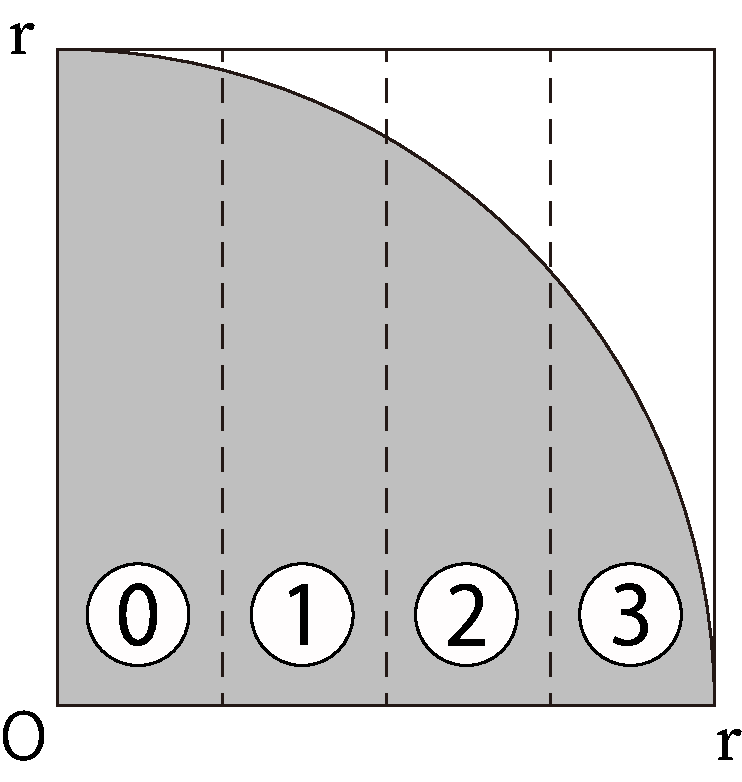
\includegraphics[width=5cm]{./images/circle.pdf}
  \caption{半径$r$の円1/4と各CPUの担当する部分}
  \label{fig:sim}
\end{figure}

\begin{align}
  n : x &= r^2 : \frac{\pi r^2}{4} \label{eq:monte} \\
  \frac{x}{n} &= \frac{\pi}{4} \notag \\
  \pi &= \frac{4x}{n}
  \label{eq:pi}
\end{align}

本プログラムでは、1/4の円をCPUの個数だけ縦に分割し、それぞれのCPUに担当させた。
例えば、4個のCPUで実行した場合は、図\ref{fig:sim}のように分担することとなる。

これらの処理を$71 \sim 77$行目で行い、80行目で各CPUで数え上げた数の集計、86行目で計算結果の算出を行っている。

\subsection{実行結果}
\subsubsection{円周率の算出}
コマンドライン引数に$2 \times 10^8$を与え、4個のCPUで実行した場合の結果をリスト\ref{lst:kadai3-1}に示す。

\lstinputlisting[style=text,caption=$2 \times 10^8$の点でのシミュレーション結果,label=lst:kadai3-1]{./MPI/result/kadai03-1.txt}

\subsubsection{並列化の効果の検証}
引数に$2 \times 10^8$を与えた場合について、CPUの数$N$を1$\sim$30個に増やしながら処理時間を測定した。
全てのCPUが作業が行われていない状態で測定を行い、それぞれ10回の平均値を取った。

それぞれのCPUの個数についての処理時間についてまとめたものを表\ref{tb:kadai3}に、グラフにプロットしたものを図\ref{fig:kadai3}に示す。

\begin{table}[htbp]
  \centering
  \caption{CPUの個数と処理時間}
  \label{tb:kadai3}

  \begin{tabular}{|r|r|r|}
    \hline
    \chuo{CPU数 [個]} & \chuo{処理時間 [ms]} & \chuo{CPU1個の処理時間に対する短縮率} \\ \hline \hline
    1 & 6895 & 1.00 \\ \hline
    2 & 3573 & 1.93 \\ \hline
    3 & 2422 & 2.85 \\ \hline
    4 & 1807 & 3.82 \\ \hline
    5 & 1438 & 4.79 \\ \hline
    6 & 1241 & 5.56 \\ \hline
    7 & 1027 & 6.72 \\ \hline
    8 & 903 & 7.63 \\ \hline
    9 & 837 & 8.24 \\ \hline
    10 & 727 & 9.48 \\ \hline
    11 & 680 & 10.15 \\ \hline
    12 & 632 & 10.91 \\ \hline
    13 & 562 & 12.26 \\ \hline
    14 & 555 & 12.42 \\ \hline
    15 & 504 & 13.67 \\ \hline
    16 & 460 & 14.98 \\ \hline
    17 & 436 & 15.81 \\ \hline
    18 & 430 & 16.02 \\ \hline
    19 & 394 & 17.49 \\ \hline
    20 & 381 & 18.12 \\ \hline
    21 & 432 & 15.95 \\ \hline
    22 & 340 & 20.27 \\ \hline
    23 & 348 & 19.82 \\ \hline
    24 & 338 & 20.43 \\ \hline
    25 & 323 & 21.36 \\ \hline
    26 & 359 & 19.20 \\ \hline
    27 & 280 & 24.64 \\ \hline
    28 & 296 & 23.27 \\ \hline
    29 & 309 & 22.34 \\ \hline
    30 & 305 & 22.60 \\ \hline
  \end{tabular}
\end{table}

\begin{figure}[H]
  \centering
  \includegraphics[width=12cm]{./MPI/kadai03-result/kadai03.png}
  \caption{CPUの個数と処理時間の関係}
  \label{fig:kadai3}
\end{figure}

\subsection{考察}
リスト\ref{lst:kadai3-1}を見ると、各CPUで違うシード値が採用されており、円周率が算出されているため、正しくモンテカルロ法によるシミュレーションが行われていると言える。

また、図\ref{tb:kadai3}を見ると、反比例のグラフであるように見える。
しかし、表\ref{tb:kadai3}を見ると、CPUを30個使用した場合の時間の短縮率は22.60と、投入した分の効果が発揮されていない。
このことから、実際に並列計算を行う場合は、投入したCPUの分だけ効率化が行えるとは限らないことが分かる。


\section{課題4}
\subsection{課題内容}
以下の処理を実行するプログラムを作成する。

\begin{enumerate}
  \item 整数配列\texttt{a[] = \{3, 1, 4, 1, 5, 9\}}をCPU 0で定義する。
  \item CPU$1 \sim 9$のそれぞれで適当な乱数\texttt{R}を1個ずつ発生させる。
  \item \texttt{a[]}を9台のCPUに\texttt{MPI\_Send}で送信し、
        受信側では\texttt{a[]}のそれぞれの要素に手順2で発生させた$R$を加えた配列\texttt{b[]}を作る。
  \item 9台のCPUからそれぞれが持っている\texttt{R}と\texttt{b}をCPU 0に送り返す。
  \item CPU 0でCPU番号とともに送り返されてきた\texttt{R}と\texttt{b}を表示する。
\end{enumerate}

\subsection{プログラムリスト}
課題4のプログラムを、リスト\ref{lst:kadai4}に示す。

\lstinputlisting[style=C,caption=課題4のプログラム,label=lst:kadai4]{./MPI/kadai04.c}

\subsection{プログラムの説明}
課題3までは、各CPUで行った計算結果に対して総和を取ったり、最大値や最小値を取得する\texttt{MPI\_Reduce}関数を使用してきた。
MPIには、これとは別に単純に値を送受信する\texttt{MPI\_Send}, \texttt{MPI\_Recv}関数が用意されている。
単一の値だけでなく、配列の送受信も行うことができ、これによりさらに自由度の高い通信が行えるようになる。

\subsection{実行結果}
課題4の実行結果をリスト\ref{lst:kadai04}に示す。

\lstinputlisting[style=text,caption=課題4の実行結果,label=lst:kadai04]{./MPI/result/kadai04-1.txt}

\subsection{考察}
リスト\ref{lst:kadai04}を見ると、各CPUについて、${3, 1, 4, 1, 5, 9}$に生成した\texttt{R}を加えた配列がCPU0に送信され、表示されている。
よって、課題内容のプログラムが正しく作成できた。


\section{課題5}
\subsection{課題内容}
シュテルマーの公式(\ref{eq:shu})を用いて円周率$\pi$を小数点以下1,000桁以上並列計算するプログラムを作成する。

\begin{equation}
  \pi = 24 \tan^{-1} \left( \frac{1}{8} \right) + 8 \tan^{-1} \left( \frac{1}{57} \right) + 4 \tan^{-1} \left( \frac{1}{239} \right)
  \label{eq:shu}
\end{equation}

\subsection{プログラムリスト}
課題5のプログラムを、リスト\ref{lst:kadai5}に示す。
なお、多倍長整数の計算には3年次で作成したライブラリを使用しているが、そのプログラムリストは省略する。
本プログラムで使っている多倍長整数ライブラリの関数とその説明をまとめたものを表\ref{tb:multiple}に示す。

\lstinputlisting[style=C,caption=課題5のプログラム,label=lst:kadai5]{./MPI/multiple/pi.c}

\begin{table}[H]
  \centering
  \caption{多倍長整数ライブラリの関数の説明}
  \label{tb:multiple}

  \begin{tabular}{|l|l|}
    \hline
    \chuo{関数名} & \chuo{説明} \\ \hline \hline
    \texttt{copyNumber} & 値をコピーする \\ \hline
    \texttt{clearByZero} & 値を0に初期化する \\ \hline
    \texttt{setInt} & 多倍長整数変数に\texttt{int}型変数の値を設定する \\ \hline
    \texttt{mulBy10} & 値を10倍する \\ \hline
    \texttt{add} & 加算を行う \\ \hline
    \texttt{multiple} & 乗算を行う \\ \hline
    \texttt{divide} & 除算を行う \\ \hline
    \texttt{dispNumber} & 多倍長整数変数の値を表示する \\ \hline
  \end{tabular}
\end{table}

\subsection{プログラムの説明}
(\ref{eq:shu})を計算するには、$\tan^{-1} x$の値が計算できれば良い。
$\tan^{-1} x$をテイラー展開すると(\ref{eq:taylor})のようになる。

\begin{equation}
  \tan^{-1} x = \sum^{\infty}_{n = 0} \frac{(-1)^n}{2n + 1} x^{2n + 1} \quad \mathrm{for} \quad |x| < 1
  \label{eq:taylor}
\end{equation}

(\ref{eq:taylor})の各項を各CPUに分担させ、計算することで並列計算を行っている。

\subsection{実行結果}
課題5の実行結果をリスト\ref{lst:kadai05}に示す。

\lstinputlisting[style=text,caption=課題5の実行結果,label=lst:kadai05]{./MPI/multiple/pi.txt}

次に、CPUの数$N$を1$\sim$30個に増やしながら処理時間を測定した。
全てのCPUが作業が行われていない状態で測定を行い、それぞれ5回の平均値を取った。

それぞれのCPUの個数についての処理時間についてまとめたものを表\ref{tb:kadai5}に、グラフにプロットしたものを図\ref{fig:kadai5}に示す。

\begin{table}[htbp]
  \centering
  \caption{CPUの個数と処理時間}
  \label{tb:kadai5}

  \begin{tabular}{|r|r|r|}
    \hline
    \chuo{CPU数 [個]} & \chuo{処理時間 [s]} & \chuo{CPU1個の処理時間に対する短縮率} \\ \hline \hline
    1 & 2165.54 & 1.00 \\ \hline
    2 & 1083.79 & 2.00 \\ \hline
    3 & 722.74 & 3.00 \\ \hline
    4 & 542.74 & 3.99 \\ \hline
    5 & 435.03 & 4.98 \\ \hline
    6 & 362.66 & 5.97 \\ \hline
    7 & 311.22 & 6.96 \\ \hline
    8 & 272.53 & 7.95 \\ \hline
    9 & 242.42 & 8.93 \\ \hline
    10 & 218.28 & 9.92 \\ \hline
    11 & 198.77 & 10.89 \\ \hline
    12 & 182.46 & 11.87 \\ \hline
    13 & 168.42 & 12.86 \\ \hline
    14 & 156.55 & 13.83 \\ \hline
    15 & 146.30 & 14.80 \\ \hline
    16 & 137.34 & 15.77 \\ \hline
    17 & 129.36 & 16.74 \\ \hline
    18 & 122.20 & 17.72 \\ \hline
    19 & 115.87 & 18.69 \\ \hline
    20 & 110.15 & 19.66 \\ \hline
    21 & 105.00 & 20.62 \\ \hline
    22 & 100.43 & 21.56 \\ \hline
    23 & 96.16 & 22.52 \\ \hline
    24 & 92.32 & 23.46 \\ \hline
    25 & 88.63 & 24.43 \\ \hline
    26 & 85.27 & 25.40 \\ \hline
    27 & 82.16 & 26.36 \\ \hline
    28 & 79.34 & 27.30 \\ \hline
    29 & 76.66 & 28.25 \\ \hline
    30 & 74.12 & 29.22 \\ \hline
  \end{tabular}
\end{table}

\begin{figure}[H]
  \centering
  \includegraphics[width=12cm]{./MPI/kadai05-result/kadai05.png}
  \caption{CPUの個数と処理時間の関係}
  \label{fig:kadai5}
\end{figure}


\subsection{考察}
まずは、正しく計算が行われていることを確認するためにマチンの公式(\ref{eq:matin})を計算するプログラムを作成した。
それをリスト\ref{lst:matin}に示す。
このプログラムの実行結果とリスト\ref{lst:kadai05}は一致したため、正しく円周率を計算できていると言える。

\begin{equation}
  \pi = 16 \tan^{-1} \left( \frac{1}{5} \right) - 4 \tan^{-1} \left( \frac{1}{239} \right)
  \label{eq:matin}
\end{equation}

\lstinputlisting[style=C,caption=マチンの公式を計算するプログラム,label=lst:matin]{./MPI/multiple/matin.c}

また、図\ref{fig:kadai5}を見ると、反比例のグラフとなっている。
さらに、表\ref{tb:kadai5}のCPU1個の処理時間に対する短縮率より、おおよそCPUの数の分だけ処理時間の短縮がされていることが分かる。
このように並列化の効果が強く出ているのは、本プログラムが通信に対して計算の比率が大きいためと考えられる。
このことから、効率的な並列計算を行うには、できるだけ通信を少なくすることが重要であることが分かる。


\section{課題6}
\subsection{課題内容}
ライフゲームを並列処理で実行するプログラムを作成する。

\subsection{プログラムリスト}
課題6のプログラムを、リスト\ref{lst:kadai6}に示す。

\lstinputlisting[style=C,caption=課題6のプログラム,label=lst:kadai6]{./MPI/LifeGame/lifegame.c}

\subsection{プログラムの説明}
本プログラムでは、ライフゲームのセルをCPUの個数だけ縦に分割している。
こうすることで、各CPUについて、通信を行うのは左右のCPUだけで済む。

\subsection{実行結果}
グライダーを初期配置として実行した結果をリスト\ref{lst:1}--\ref{lst:5}に示す。

\lstinputlisting[style=text,caption=グライダーの第0世代,label=lst:1]{./MPI/LifeGame/1.txt}

\lstinputlisting[style=text,caption=グライダーの第1世代,label=lst:2]{./MPI/LifeGame/2.txt}

\lstinputlisting[style=text,caption=グライダーの第2世代,label=lst:3]{./MPI/LifeGame/3.txt}

\lstinputlisting[style=text,caption=グライダーの第3世代,label=lst:4]{./MPI/LifeGame/4.txt}

\lstinputlisting[style=text,caption=グライダーの第4世代,label=lst:5]{./MPI/LifeGame/5.txt}

次に、ランダムなセルの状態から10000世代実行するプログラムで、CPUの数$N$を1$\sim$30個に増やしながら処理時間を測定した。
全てのCPUが作業が行われていない状態で測定を行い、それぞれ10回の平均値を取った。

それぞれのCPUの個数についての処理時間についてまとめたものを表\ref{tb:kadai6}に、グラフにプロットしたものを図\ref{fig:kadai6}に示す。

\begin{table}[htbp]
  \centering
  \caption{CPUの個数と処理時間}
  \label{tb:kadai6}

  \begin{tabular}{|r|r|r|}
    \hline
    \chuo{CPU数 [個]} & \chuo{処理時間 [s]} & \chuo{CPU1個の処理時間に対する短縮率} \\ \hline \hline
    1 & 154.46 & 1.00 \\ \hline
    2 & 77.82 & 1.98 \\ \hline
    3 & 52.15 & 2.96 \\ \hline
    4 & 39.82 & 3.88 \\ \hline
    5 & 32.37 & 4.77 \\ \hline
    6 & 27.01 & 5.72 \\ \hline
    7 & 23.35 & 6.62 \\ \hline
    8 & 20.57 & 7.51 \\ \hline
    9 & 18.60 & 8.31 \\ \hline
    10 & 16.80 & 9.19 \\ \hline
    11 & 15.49 & 9.97 \\ \hline
    12 & 14.34 & 10.77 \\ \hline
    13 & 13.25 & 11.66 \\ \hline
    14 & 12.34 & 12.51 \\ \hline
    15 & 11.60 & 13.32 \\ \hline
    16 & 11.07 & 13.95 \\ \hline
    17 & 10.62 & 14.55 \\ \hline
    18 & 10.21 & 15.13 \\ \hline
    19 & 9.68 & 15.95 \\ \hline
    20 & 9.21 & 16.77 \\ \hline
    21 & 8.91 & 17.34 \\ \hline
    22 & 8.65 & 17.86 \\ \hline
    23 & 8.31 & 18.59 \\ \hline
    24 & 8.03 & 19.24 \\ \hline
    25 & 7.78 & 19.84 \\ \hline
    26 & 7.58 & 20.39 \\ \hline
    27 & 7.31 & 21.13 \\ \hline
    28 & 7.15 & 21.61 \\ \hline
    29 & 6.91 & 22.34 \\ \hline
    30 & 6.75 & 22.90 \\ \hline
  \end{tabular}
\end{table}

\begin{figure}[H]
  \centering
  \includegraphics[width=12cm]{./MPI/kadai06-result/kadai06.png}
  \caption{CPUの個数と処理時間の関係}
  \label{fig:kadai6}
\end{figure}

\subsection{考察}
リスト\ref{lst:1}--\ref{lst:5}を見ると、4世代後に初期と同じ形状になり、初期地点から1つ右下に移動していることが分かる。
よって、正しくグライダーを飛ばすことができたため、ライフゲームのプログラムを作成することができた。

また、図\ref{tb:kadai6}を見ると、反比例のグラフであるように見える。
しかし、表\ref{tb:kadai6}を見ると、使用したCPUの個数に対してあまり効率化は行われていない。
このことから、本プログラムのような通信が多い並列処理では、並列処理の恩恵を受けづらいと言える。


\begin{thebibliography}{9}
  \bibitem{bib:1} OpenMPI: Open Source High Performance Computing, \texttt{\url{https://www.open-mpi.org/}}
  \bibitem{bib:2} MPICH $|$ High-Performance Portable MPI, \texttt{\url{https://www.mpich.org/}}
\end{thebibliography}


\end{document}
